\subsection{Why A and B must remain ordered}
The contest supplies an ideal cubic prototype. To isolate the effect of site assignment in the illustration, we hold its fractional coordinates fixed and place A at the corners, B at the body center and the anions at the face centers \cite{aflow}. The eight corners contribute $8/8=1$ A atom per cell. The six faces contribute $6/2=3$ anions. B has six nearest anion neighbors in the illustrated octahedron, while the periodically repeated face centers give A twelve nearest anion neighbors. The contest family label specifies the composition of the three anions. For example, NO2 supplies one N and two O per formula unit. For the blind candidate this fixes stoichiometry only; the data leave the O/N site ordering unresolved.

Figure~\ref{fig:cell} compares two DFT records at reversed site assignments. The exchange arrow connects two separately calculated compositions.

\begin{figure}[htbp]
\centering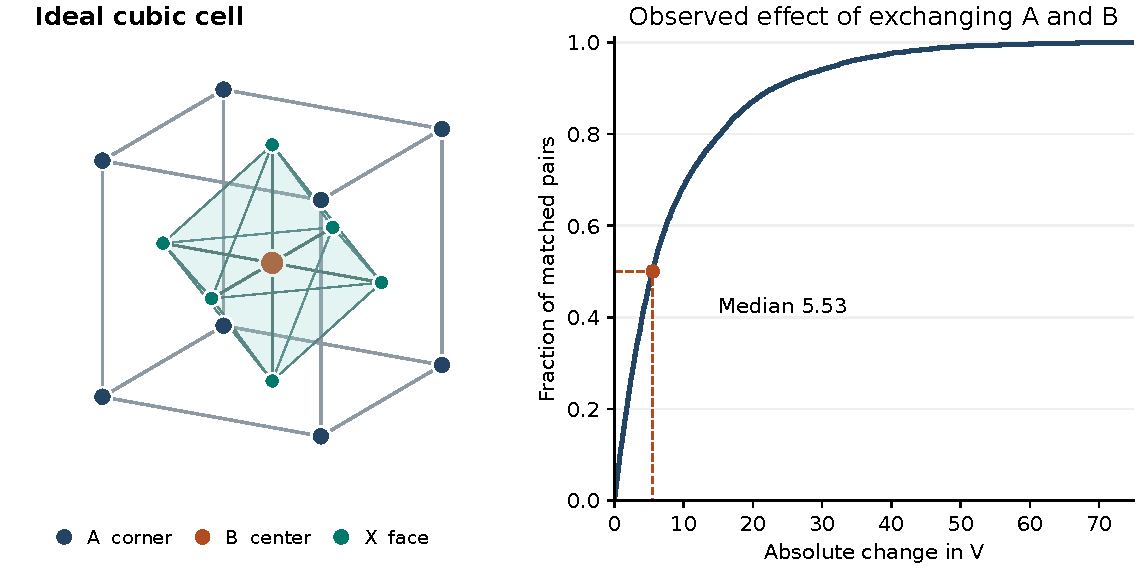
\includegraphics[width=.98\linewidth]{figures/crystal_sites.pdf}
\caption{Exchanging the corner and central cations in the ideal cubic prototype \cite{aflow}. Gap and violation are the public DFT values for each composition.}\label{fig:cell}
\end{figure}

We matched each public record $(a,b,x)$ with $(b,a,x)$ when both were labeled, excluded $a=b$, and counted each reciprocal pair once. Among 5,971 matches, the median absolute difference is 5.5296, with quartiles 2.2672 and 12.6046. A predictor that gives both records the same output $h$ incurs
\[
 \tfrac12\{|V(a,b,x)-h|+|V(b,a,x)-h|\}\ \geq\
 \tfrac12 |V(a,b,x)-V(b,a,x)|.
\]
Averaging the right-hand side gives an unavoidable MAE of at least 4.6805 on these 11,942 matched rows for a site-invariant predictor. This bound concerns the matched sample and must be compared on that same sample. It motivates retaining separate A and B descriptors before fitting.

The Sn--Ti pair illustrates the size of this effect. Public $\mathrm{SnTiO_3}$ has $g=2.50$ eV and $V=0.001419$. Its reversed assignment $\mathrm{TiSnO_3}$ has $g=0$ and $V=18.422244$. For $\mathrm{SnTiO_3}$ the supplied cubic lattice parameter is 3.969143~\AA. Lattice parameters and volumes are available only in labeled records and do not enter the score of a new composition.
